\chapter{Hackystat-Trajectory - software process mining framework.} \label{trajectory}
As we saw in the Chapter \ref{related.work} it is possible to infer and successively formalize software process by observing its artifacts, and particularly, recurrent behavioral patterns. The problem of finding such patterns is the cornerstone of my research. My approach to this problem rests on the application of data-mining techniques to symbolic time-point and time-interval series constructed directly from the real-valued telemetry streams provided by Hackystat.

\begin{figure}[tbp]
   \centering
   \includegraphics[height=65mm]{system_overview.eps}
   \caption{The high-level system overview. Software engineering process and product data collected and aggregated by Hackystat used to generate temporal symbolic indexes. Data mining tools constrained by the software engineering domain knowledge are then used for unsupervised patterns discovery. The GUI provides an expert interface for discovered patterns and knowledge base aiding iterative investigation of a discovered phenomena.}
   \label{fig:system_overview}
\end{figure}


Aiming the delivery of a software tool aiding in discovery of recurrent behavioral patterns in software process, I am designing and developing a ``Hackystat Trajectory'' framework, which provides an ``one-stop shop'' for recurrent behavior patterns mining from software process data. The high-level overview of the framework is shown at the Figure \ref{fig:system_overview} and resembles the flow of the Knowledge Discovery in Database process discussed by Han et al. in \cite{citeulike:709476}. As shown, the data collected by Hackystat are getting transformed into a symbolic format and then indexed for further use in the data-mining. The tools, designed for data-mining, have a specific restrictions placed on the search space by domain and context knowledge in order to limit the amount of reported patterns to the useful ones. I am planning to design a GUI in a way which will allow easy access and modification of these rules. 

\section{Current state of the development}
I have started development of the Hackystat Trajectory framework in early 2008 by designing a user interface for visual comparison of multi-variate time series. This was done by following the idea expressed by Philip Johnson which he called as ``From Telemetry to Trajectory''. Borrowing the term ``trajectory'' I have called the software package as ``TrajectoryBrowser'' and titled performed analysis as ``Software Trajectory Analysis''. The idea was to visualize software project metrics as a set of trajectories in 3D space, as an opposite to the classical 2D representation. The first \textit{TrajectoryBrowser} was an ad-hoc application based on the two technologies: Java3D for visualization and UI and JADE multi-agent framework \cite{citeulike:1230319} for the data generation (see Figure \ref{fig:trajectory_progress} panels $a$ and $b$). While this first version fulfilled basic requirements for visualization, allowing trajectories ``eyeballing'', it did not provide any means for quantifying similarities between trajectories or finding similar trajectories autonomously.

In order to introduce a metric and implement an indexing of temporal features, I have started experimenting with a naive application of Euclidean distance and later with spectral decomposition of time series through DFT. Unfortunately both methods were found inconsistent in results and sometimes even misleading due to the noisy and bursty nature of temporal data generated by the software process. 

\begin{figure}[tbp]
   \centering
   \includegraphics[height=155mm]{trajectory_progress.eps}
   \caption{Screenshots of three versions of TrajectoryBrowser (panels $a$, $b$ and $d$) and the software process simulation (panel $b$). Simulated data was used for validation in early stages.}
   \label{fig:trajectory_progress}
\end{figure}

At the next iteration, inspired by a success in many applications and robustness to noise, I have implemented Dynamic Time Warping (DTW) algorithm. This code was wrapped into the second, web-based version of TrajectoryBrowser (see Figure \ref{fig:trajectory_progress} panels $c$). The second version provided a user with ability to visualize time-series intervals and quantify the similarity. Nevertheless, there was no implementation of the unsupervised similarity search provided.

Aiming closing this gap, I have started developing the indexing module by using sliding window and DTW. While working on this, I found another promising approach for the same task: PAA and SAX (see section \ref{paa} and \ref{sax}) approximations. The simplicity of these two methods allowed me to integrate them with my existed codebase almost instantly, delivering the third version of TrajectoryBrowser which I am currently using in my research. Next two sub-section will present the indexing mechanism and the index database design. 

\subsection{Temporal data indexing}
The temporal data indexing starts with the data abstraction process shown at the Figure \ref{fig:data_flow}. Collected and aggregated by Hackystat, \textit{raw sensor data} and derived \textit{Hackystat Telemetry streams} are used as the data sources. Streams of individual events are retrieved from Hackystat Sensorbase then sorted by activity types, tokenized, and finally converted into symbolic time point (\textit{Events}) and time-interval (\textit{Episodes}) series by following a user-defined taxonomy mapping. By performing a user-configured PAA and successive SAX approximations, Hackystat Telemetry streams are getting converted into the same temporal symbolic format. This symbolic data, in turn, are getting indexed and stored in the dedicated relational database for future use in data mining.

\begin{figure}[tbp]
   \centering
   \includegraphics[height=85mm]{data_flow.eps}
   \caption{The overview of the data abstraction from the the low-level process and product artifacts collected by Hackystat (left side) to the high-level symbolic time-point and time-interval series stored in the Trajectory data repository.}
   \label{fig:data_flow}
\end{figure}

I have not experimented with symbolic abstraction and mining of the raw sensor data yet, but this approach has a solid foundation provided by Hongbing Kou, in his thesis \cite{citeulike:2703162}. In his work, he was able to infer TDD behaviors by using a technique called Software Development Stream Analysis (SDSA) which is very similar to mine. Within SDSA, the low-level software process data was converted into symbolic Episodes first. At the second step, sequences of Episodes (candidate patterns) were matched to the set of the known TDD temporal rules (patterns), and if they were found satisfying TDD rules (having sufficient support), the generative process was inferred as TDD.

The indexing of Telemetry streams I have implemented with sliding window, PAA, and SAX. I am using a sliding window approach following \cite{citeulike:2821475} for generating a set of subsequences from a real-valued stream. Each of subsequences then getting normalized and converted into symbolic representation with PAA and SAX. This symbolic representation and the position information then stored in the relational database. For index manipulation and data retrieval I am leveraging SQL. Figure \ref{fig:indexer} presents the current software system overview.

\subsection{Index database design}
Figure \ref{fig:trajectory_db} presents the TrajectoryDB database schema in detail. This schema was designed with two main requirements in mind. First of all, it must be able to hold a local copy of Telemetry streams due to the high time cost of querying Telemetry service remotely. Secondly, it must support implemented KDD algorithms through optimized for speed SQL queries. Both goals were archived, resulting in the extremely high turn-around speed for both, indexing and querying.

\begin{figure}[tbp]
   \centering
   \includegraphics[height=60mm]{indexer.eps}
   \caption{Overview of the current implementation of Hackystat Trajectory framework.}
   \label{fig:indexer}
\end{figure}

Current version of Hackystat is implemented based on the Service-Oriented architecture, and in order to retrieve a Telemetry data one must query Telemetry service over network. My initial implementation of the indexing was performing network queries for the each of the indexing passes and was significantly affected by the network lag for my remote location and the amount of data needed to be retrieved for each pass. To overcome this issue I have developed a software module which is ``caching'' and incrementally updating Telemetry streams data locally. The \textit{Project, User, Member, Chart, Chartvalue} and \textit{Download} tables (located at the upper part of the Figure \ref{fig:trajectory_db}) are designed to store the Telemetry data locally. The system performs incremental update of the streams over the time by reading the \textit{Download} table, which keeps track of updates.

The telemetry streams indexing is performed on demand. For each of the indexes a sliding window size, PAA size, and an alphabet must be specified. Following Lin \& Keogh \cite{citeulike:2821475}, in order to investigate the sensitivity and selectivity of different approximation levels, I have conducted a number of experiments with various alphabets. Individual alphabets for each of the data streams (\textit{Build, Coverage} etc.) and \textit{Universal Telemetry Alphabet} (see example for five letters alphabet at the Figure \ref{fig:distribution}, panel $a$) were built and tested for indexing. These custom alphabets, and the original SAX alphabet, based on the Normal distribution, are kept in the \textit{Sax\_alphabet} and \textit{Alphabet\_cut} tables. 

The \textit{Sax\_top\_index} table is a ``binder'' which keeps information about all indexes ever built. The \textit{Sax\_index\_chart} table keeps track of all indexes built for a particular chart and a timeframe. \textit{Sax\_motif} and \textit{Sax\_motif\_entry} tables separate heavyweight symbolic motifs and lightweight offset ``information'' reducing the database size and optimizing data analysis and retrieval. 

This database schema was found optimal for easy retrieval of any kind of information needed for streams comparisons or clustering. By running a single query it is possible to retrieve a vector of most frequent motifs for each of the streams or find a set of motifs shared between streams.

\section{TrajectoryBrowser}
As mentioned before, the current version of TrajectoryBrowser was created in order to visualize telemetry streams along with temporal features found through indexing. It provides easy navigation within indexes and capable of displaying multiple telemetry streams with highlighted features. By viewing the same motif entry across multiple streams it is possible to guess information about coincidence of entries, as an example, see Section \ref{pilot.evaluation}, for sequential ``growth'' pattern finding experiment.

\section{Future development roadmap}
As I pointed before, the current version of the TrajectoryBrowser and analyses do not support processing of the low-level raw Hakystat data and based on it analyses. I have already started the development of such module along with extending a database schema for storing raw data, its approximation, and taxonomy. Once all this components will be in place, I will start developing data mining algorithms for Events and Episodes using discussed temporal data mining algorithms. Once all major software pieces will be in place, I will focus on the experimental evaluation of the system and improving the usability of the GUI.